% Drawing 144/04-5 -- folder 144, batch 04, archive page 64 (PDF page 65).
% Transcription: (24) Dans la marge, une sphère : $P_+$ au pôle nord ; trois demi-méridiens $\lambda_0$, $\lambda_1$, $\lambda_\infty$ qui y aboutissent, passant par $Q_0 = 2$, $Q_1 = -1$, $Q_\infty = \tfrac12$ ; les points $0$, $1$, $\infty$ sur l'équateur ; des parties des arcs en pointillé.
% Kind: sphere with three half-meridians through Q_0, Q_1, Q_infty. Method 2 (schematic redraw from the facsimile). Status: ok.
% Notes: Pencil outline of the sphere and pencil equator. The three half-meridians are drawn from the north pole P_+ through the points Q where they cross the equator (each Q computed on the equator, the meridian passing exactly through it) and down to the south pole, where they meet: lambda_1 on the left, dotted as on the page; lambda_infty in the middle, solid; lambda_0 on the right, dotted. The three big dots are on the equator (back, front left, front right). Labels \small where he wrote them: P_+, lambda_1, lambda_infty, lambda_0, Q_1 = -1, Q_0 = 2, Q_infty = 1/2. The bbox now takes in the whole sphere; the (24) under it and the word at the top are not drawn. Redrawn 2026-11-09 (issue 128): to check again. Question settled by a machine pass on the facsimile, 2026-11-12 (page): at 600 dpi the back dot carries a small infinity above it, the front left dot a 0 and the front right dot a 1 under it, which agrees with Q_infty = 1/2 lying between 0 and 1, Q_1 = -1 between infinity and 0 and Q_0 = 2 between 1 and infinity; the three labels are added. Not checked by a reader. Overlay check 2026-11-13 (issue 147, Claude Opus 5.5): the redraw, rasterised from its TikZ paths, laid over the 300 dpi colour render of the 250 ppi scan with the contrast raised, since the outline and the equator are faint pencil. Redrawn from the page: the outline is no longer an ellipse but a closed curve through points read on its pencil (flattened at the upper right, widest at the right); the equator is the tilted pencil ellipse of the page, its back arc through the back dot (which now sits on it, where it is on the page) and its front arc just above the two front dots; lambda_1 and lambda_0 dotted, each through the dots of the page; lambda_infty solid from P_+ to the south pole (below Q_infty it is a solid stroke on the page, not dashed); the two short pencil strokes inside the lower left of the sphere are drawn; the labels were moved onto their ink. Every stroke lies on its ink to within about 1 unit. Not compiled (no TeX engine in the session).
% Coordinates: 1 unit = 1 mm = 1/100 of the crop width (bbox in page fractions: [0.08, 0.69, 0.3, 0.84]).
% Redrawn by Claude (claude-opus-5-5), issue #73, 2026-11-09; not checked by a human; not compiled (no TeX in the session).
% Checked by Claude (claude-opus-5-5) 2026-11-13 (issue #147): overlay on the 300 dpi colour render of the 250 ppi scan (contrast raised for the pencil), redrawn; not compiled (no TeX in the session). Not checked by a human. Status: ok.
% Rights: reproduces part of the work -- behind RENDER_TRANSCRIPTS, never published by itself.
\documentclass[tikz,border=3pt]{standalone}
\usepackage{amsmath,amssymb}
\usetikzlibrary{patterns,arrows.meta}
\tikzset{pencil/.style={black!45}, struck/.style={black!35}, mark/.style={circle,draw,inner sep=1.3pt}, pt/.style={circle,fill,inner sep=0.9pt}, opt/.style={circle,draw,fill=white,inner sep=1.1pt}}
\begin{document}
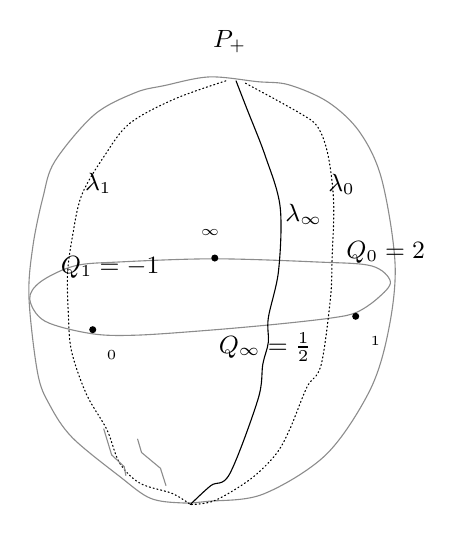
\begin{tikzpicture}[x=1mm,y=1mm,line cap=round,line join=round,font=\scriptsize]
\draw[pencil] plot[smooth cycle, tension=0.55] coordinates {(56.4,-30) (62.5,-30.6) (66.5,-31) (71.5,-33.2) (75.5,-37) (78.3,-43) (80,-53.8) (79.1,-62.5) (76.7,-70) (71.2,-78) (63.2,-83) (56.2,-83.9) (52.9,-84.1) (48.9,-83.5) (45.1,-80.8) (39,-75.8) (36.1,-71.6) (34.6,-67.6) (33.5,-58) (34,-51.5) (35.3,-45.2) (36.8,-40.7) (41.8,-34.8) (47,-32) (50.7,-31.1)};
\draw[pencil] plot[smooth cycle, tension=0.55] coordinates {(33.6,-58.2) (35.5,-61) (41.4,-62.6) (47,-62.8) (56,-62.2) (65,-61.4) (72,-60.6) (75.1,-59.9) (77.8,-58.1) (79.4,-56) (77,-54) (70,-53.5) (57,-53.1) (45,-53.5) (39.3,-54) (35,-56)};
\draw[densely dotted] plot[smooth, tension=0.55] coordinates {(58.5,-30.5) (52,-32.8) (46.3,-35.9) (43.1,-40) (40.2,-45) (39,-50.4) (38.4,-55) (38.5,-60) (38.9,-64.8) (40.8,-70.3) (43.4,-74.8) (45,-79) (47.6,-81.6) (51.7,-82.9) (54,-84.3)};
\draw plot[smooth, tension=0.55] coordinates {(59.8,-30.5) (61.2,-34.1) (63.5,-40) (65.4,-46.5) (65.2,-54.6) (63.9,-60.6) (63.9,-63.7) (63.2,-66.5) (62.6,-70.9) (59,-80.4) (56.6,-81.9) (54,-84.3)};
\draw[densely dotted] plot[smooth, tension=0.55] coordinates {(61,-30.8) (67.9,-34.6) (70.2,-36.4) (71.5,-40) (72.2,-46) (72,-53) (71.8,-58) (70.6,-66.6) (68.8,-69.4) (66.6,-74.8) (64.8,-78) (61.6,-81.1) (57.1,-83.8) (54,-84.3)};
\draw[pencil] (43,-74.7) -- (44,-78) -- (45.6,-79.5) -- (45.8,-80.6);
\draw[pencil] (47.3,-76) -- (47.8,-77.7) -- (50.2,-79.7) -- (50.9,-81.9);
\node[pt] at (57.1,-53) {};
\node[pt] at (41.6,-62.1) {};
\node[pt] at (75,-60.4) {};
\node[inner sep=1pt] at (59,-25.5) {\small $P_+$};
\node[inner sep=1pt] at (56.5,-49.8) {\tiny $\infty$};
\node[inner sep=1pt] at (44,-65.3) {\tiny $0$};
\node[inner sep=1pt] at (77.5,-63.5) {\tiny $1$};
\node[inner sep=1pt] at (42.3,-43.5) {\small $\lambda_1$};
\node[inner sep=1pt] at (68.4,-47.5) {\small $\lambda_\infty$};
\node[inner sep=1pt] at (73.2,-43.6) {\small $\lambda_0$};
\node[inner sep=1pt] at (43.8,-54.2) {\small $Q_1=-1$};
\node[inner sep=1pt] at (78.8,-52.3) {\small $Q_0=2$};
\node[inner sep=1pt] at (63.5,-64.3) {\small $Q_\infty=\tfrac12$};
\end{tikzpicture}
\end{document}
